\subsection{Misspecified neighbourhoods, heterogeneity and exposure definition (H3, H4)}
\textbf{Omitted multi-hop spillover.} Under the linear-in-means equilibrium the one-hop regression misses everything beyond one hop, and its bias follows Prop.~\ref{prop:mh} (Fig.~\ref{fig:mh}a; Appendix Table~\ref{tab:mh}): on ER ($d{=}30$) at $\lambda=0.6$ the simulated bias is $-0.872\pm0.007$ (s.e.\ over worlds) against $-0.867$ (exact walk-statistics formula) and $-0.900$ (tree-like approximation), a $35\%$ relative error of a GATE of $2.49$ independent of $n$; at $\lambda=0.8$ it is $63\%$. On triangle-rich ego-Facebook the tree-like formula fails ($-0.900$ vs simulated $-0.710$) but the exact one, using the graph's return/closure statistics $\psi_k$, does not ($-0.696$); on Stanford3 both agree ($-0.850$ exact vs $-0.846$). Adding the two-step exposure $s^{(2)}$ reduces the bias (ER, $\lambda{=}0.6$: $-0.87\to-0.55$; the rest comes from hops $\ge3$) but multiplies the SD by $5.4$ (ER), $4.0$ (Stanford3), $2.3$ (ego-Facebook) under Bernoulli ($\lambda{=}0.4$; leverage $3560$ vs $121$ on ER), so its RMSE is higher than the one-hop model's in 6 of 7 graph/design combinations at $\lambda=0.4$ and lower in 4 of 7 at $\lambda=0.6$ (all on real graphs). \textbf{Cluster randomization absorbs part of the omitted effect:} at $\lambda=0.6$ the bias falls from $-0.71$ to $-0.11$ on ego-Facebook, $-0.85$ to $-0.49$ on Stanford3, $-0.86$ to $-0.67$ on SBM, and grows again as clusters get finer (Fig.~\ref{fig:des}f).

\begin{figure}[t]
\centering
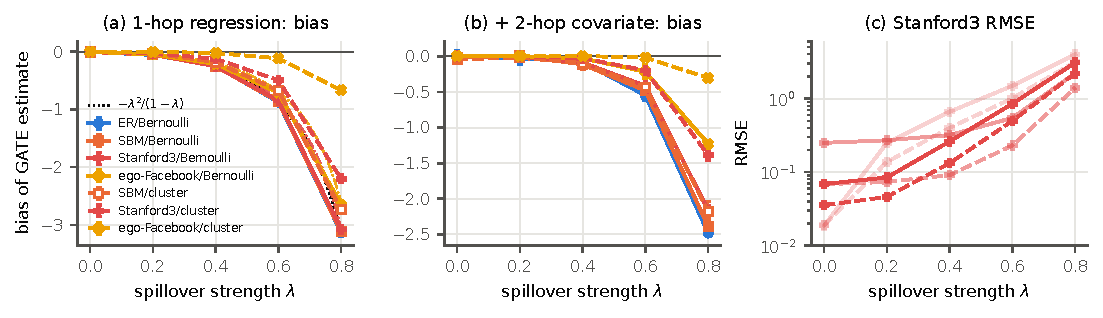
\includegraphics[width=\linewidth]{figs/fig_multihop.pdf}
\caption{Multi-hop interference (E3). (a) Bias of the one-hop regression vs $\lambda$ under Bernoulli (solid) and cluster designs (dashed) on four graphs; dotted black: tree-like prediction $-\lambda^2/(1-\lambda)$; dash-dotted: exact formula of Prop.~\ref{prop:mh} for ego-Facebook (yellow) and Stanford3 (red). (b) Bias after adding the two-step exposure. (c) RMSE on Stanford3: one-hop regression (dark), two-step regression (mid), DiM (light); solid Bernoulli, dashed cluster. Mean over 6 worlds, bars min--max.}
\label{fig:mh}
\end{figure}


\textbf{Heterogeneous susceptibility.} If $\gamma_i$ depends on degree, \textsc{ols-s} converges to a $1/d_i$-weighted average of unit effects (Prop.~\ref{prop:wt}; Table~\ref{tab:het}). On Stanford3 with ``inv'' heterogeneity (GATE $2.0$) the bias is $+2.04$ -- the estimate is twice the truth -- as predicted ($+2.03$, evaluated on the actual world parameters; per-world predictions and simulations agree within $0.02$); ``pos'': $-0.71$ ($-0.71$); ego-Facebook $+1.41$ ($+1.41$) and $-0.60$ ($-0.59$); BA graphs, with less degree spread, $+0.17$ and $-0.40$. Without degree-related heterogeneity it is unbiased ($|$bias$|\le0.01$). Adding the neighbour count or $s\times$log-degree reduces but does not remove the bias ($+1.55$, $-0.53$ on Stanford3 ``inv''). Variance-weighted fitting (\textsc{wls-s}) removes it ($+0.02$) but with RMSE $0.19$--$0.64$ (vs $0.07$--$0.12$ for \textsc{ols-s} in the homogeneous case); degree stratification (\textsc{strat-s}) gives bias $+0.20$, RMSE $0.27$ (vs $2.04$) and is almost free under cluster randomization (RMSE $0.04$--$0.05$). Both were devised after the pilot results.

\textbf{Exposure definition.} If spillover follows the neighbour \emph{count} (scaled by mean degree) but the model uses the \emph{fraction}, \textsc{ols-s} is biased by $-0.90$ (Stanford3) and $-0.75$ (ego-Facebook); the converse mismatch gives $-0.98$ and $-0.97$ (RMSE $0.98$). Including both $s$ and $c$ fixes both directions (RMSE $0.07$/$0.12$ under the fraction and $0.07$/$0.13$ under the count mechanism, vs $0.03$/$0.06$ for the correct count model), provided the true exposure is nested in the model.

\begin{table}[t]\centering\footnotesize\setlength{\tabcolsep}{3pt}
\caption{Degree-heterogeneous spillover (E3): bias (RMSE); true GATE $\approx2$. ``inv'': low-degree units are more susceptible, ``pos'': high-degree units. $B$: bias predicted by Prop.~\ref{prop:wt} for \textsc{ols-s}. $+c$: model with $s$ and the neighbour count; \textsc{s-deg}: $s$ and $s\times$log-degree; \textsc{wls-s}: weights $1/\mathrm{Var}(s_i)$; \textsc{strat-s}: separate fits in 5 degree strata (the last two designed after the pilot, see text). Mean over 6 worlds.}
\label{tab:het}
\begin{tabular}{lllcccccc}\toprule
graph & $\gamma_i$ het. & design & $B$ (Prop.~\ref{prop:wt}) & \textsc{ols-s} & $+c$ & \textsc{s-deg} & \textsc{wls-s} & \textsc{strat-s} \\
\midrule
Stanford3 & none & Bern. & -0.00 & -0.01 (0.07) & +0.00 (0.07) & +0.01 (0.16) & +0.00 (0.19) & +0.00 (0.19) \\
 &  & cluster & -- & -0.00 (0.04) & +0.00 (0.04) & -0.00 (0.04) & -0.00 (0.05) & +0.00 (0.04) \\
 & inv & Bern. & +2.03 & +2.04 (2.04) & +1.55 (1.56) & -0.53 (0.56) & +0.02 (0.21) & +0.20 (0.27) \\
 &  & cluster & -- & +0.65 (0.70) & +0.35 (0.37) & -0.08 (0.13) & +0.21 (0.30) & +0.08 (0.09) \\
 & pos & Bern. & -0.71 & -0.71 (0.71) & -0.25 (0.26) & -0.18 (0.24) & +0.00 (0.26) & -0.04 (0.21) \\
 &  & cluster & -- & -0.34 (0.38) & -0.07 (0.09) & -0.05 (0.07) & -0.14 (0.24) & -0.02 (0.05) \\
\midrule
ego-Facebook & none & Bern. & -0.00 & -0.00 (0.12) & +0.01 (0.12) & +0.00 (0.19) & +0.01 (0.23) & +0.00 (0.24) \\
 &  & cluster & -- & +0.01 (0.04) & +0.01 (0.04) & +0.01 (0.04) & +0.00 (0.04) & +0.01 (0.05) \\
 & inv & Bern. & +1.41 & +1.41 (1.52) & +1.13 (1.22) & -0.44 (0.52) & +0.03 (0.36) & +0.18 (0.31) \\
 &  & cluster & -- & +0.06 (0.15) & +0.01 (0.09) & -0.01 (0.07) & +0.02 (0.15) & +0.02 (0.05) \\
 & pos & Bern. & -0.59 & -0.60 (0.65) & -0.17 (0.21) & -0.19 (0.30) & -0.05 (0.64) & -0.07 (0.30) \\
 &  & cluster & -- & -0.04 (0.16) & +0.01 (0.05) & -0.01 (0.07) & -0.01 (0.18) & -0.01 (0.06) \\
\bottomrule\end{tabular}\end{table}


\subsection{Design: treated fraction and clustering (H5)}
Under Bernoulli designs RMSE scales as $(p(1-p))^{-1/2}$ (Fig.~\ref{fig:des}a): the RMSE at $p=0.05$ is $2.2$, $2.3$, $2.2$ times that at $p=0.5$ on SBM, ego-Facebook, Stanford3 against a predicted $2.29$, and $\hat\kappa\sqrt{L/n}$ matches all runs of this sweep (median ratio $0.97$, range $[0.81,1.21]$). The bias under nonlinear response also depends on $p$ (Fig.~\ref{fig:des}b,c): with a concave response a small $p$ gives a large positive bias ($+1.7$ on SBM at $p{=}0.05$, $k{=}\frac12$) whose sign flips near $p\approx0.3$--$0.5$, agreeing with Prop.~\ref{prop:extrap} to a median of $0.011$--$0.014$ (max $0.14$--$0.21$ at $p=0.05$, where few units are treated). Small treated fractions, typical of cautious rollouts, are thus both noisier and more extrapolation-prone.

The number of clusters trades bias against variance (Fig.~\ref{fig:des}d--f). Finer clusters cut more edges, so the bias from nonlinear response and omitted hops grows monotonically (ego-Facebook $k{=}4$: $0.00\to-0.08$ from 7 to 559 clusters; Stanford3 multi-hop: $-0.28\to-0.62$), while very few clusters leave few independent units (Stanford3: RMSE $0.15$ with 5 clusters, one holding $87\%$ of units, vs $0.035$ with $\approx18$). For a linear response RMSE is flat from $\approx10$ (ego-Facebook; $0.04$--$0.05$) or $\approx18$ (Stanford3; $0.035$--$0.045$) to 600 clusters, with a shallow minimum near 80 on SBM; with a nonlinear response fewer clusters are preferred (SBM $k{=}4$: $0.34$ at 40 clusters vs $0.46$ at 690). With 30 clusters DiM remains biased by $-0.14$ ($7\%$ of the GATE) on ego-Facebook and $-0.50$ ($25\%$) on Stanford3, so clustering alone does not remove the need for the regression correction.

\begin{figure}[t]
\centering
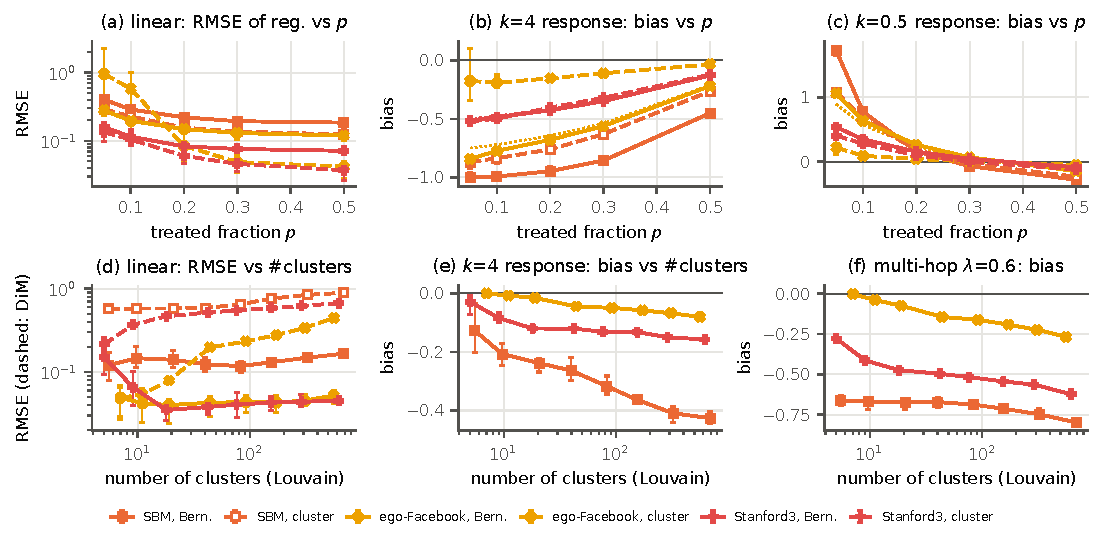
\includegraphics[width=\linewidth]{figs/fig_design.pdf}
\caption{Design factors (E5), \textsc{ols-s} estimator. Top: treated fraction $p$ (solid Bernoulli; dashed cluster randomization with $\approx$30/40 clusters; dotted: closed-form bias for Bernoulli). Bottom: number of clusters (same colours/markers per graph; solid: \textsc{ols-s}, dashed in (d): DiM). Mean over 6 worlds, bars min--max.}
\label{fig:des}
\end{figure}
